\subsection{Диффракция}

Электромагнитное излучение берет свое название из принципа переноса энергии, который происходит в следствие колебаний электрического и магнитного полей. В случае одномерных гармонических колебаний уравнения Максвелла имеют такое решение:
\begin{align*}
	\vec E(x, t) &= \vec E_0 \cos (k x - \omega t + \varphi_0),\\
	\vec H(x, t) &= \vec H_0 \cos (k x - \omega t + \varphi_0).
\end{align*}
\begin{wrapfigure}{l}{0.45\tw}
	\centering
	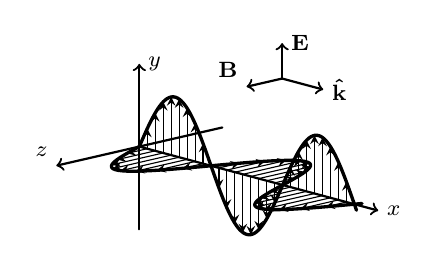
\begin{tikzpicture}[x=(-15:1.2), y=(90:1.0), z=(-150:1.0),
		line cap=round, line join=round,
		axis/.style={black, thick,->},
		vector/.style={>=stealth,->}, scale=0.5]
		\footnotesize
		\def\A{1.5}
		\def\nNodes{3} % use even number
		\def\nVectorsPerNode{8}
		\def\N{\nNodes*40}
		\def\xmax{\nNodes*pi/2*1.01}
		\pgfmathsetmacro\nVectors{(\nVectorsPerNode+1)*\nNodes}
		
		\def\vE{\mathbf{E}}
		\def\vB{\mathbf{B}}
		\def\vk{\mathbf{\hat{k}}}
		
		% main axes
		\draw[axis] (0,0,0) -- ++(\xmax*1.1,0,0) node[right] {$x$};
		\draw[axis] (0,-\A*1.4,0) -- (0,\A*1.4,0) node[right] {$y$};
		\draw[axis] (0,0,-\A*1.4) -- (0,0,\A*1.4) node[above left] {$z$};
		
		% small axes
		\def\xOffset{{(\nNodes-2)*pi/2}}
		\def\yOffset{\A*1.2}
		\def\zOffset{\A*1.2}
		\draw[axis] (\xOffset,\yOffset,-\zOffset) -- ++(\A*0.6,0,0) node[right] {$\vk$};
		\draw[axis] (\xOffset,\yOffset,-\zOffset) -- ++(0,\A*0.6,0) node[right] {$\vE$};
		\draw[axis] (\xOffset,\yOffset,-\zOffset) -- ++(0,0,\A*0.6) node[above left] {$\vB$};
		
		% waves
		\draw[very thick,variable=\t,domain=0:\nNodes*pi/2*1.01,samples=\N]
		plot (\t,{\A*sin(\t*360/pi)},0);
		\draw[very thick,variable=\t,domain=0:\nNodes*pi/2*1.01,samples=\N]
		plot (\t,0,{\A*sin(\t*360/pi)});
		
		% draw vectors
		\foreach \k [evaluate={\t=\k*pi/2/(\nVectorsPerNode+1);
		\angle=\k*90/(\nVectorsPerNode+1);
		\c=(mod(\angle,90)!=0);}]
		in {1,...,\nVectors}{
		\if\c1
		\draw[vector] (\t,0,0) -- ++(0,{\A*sin(2*\angle)},0);
		\draw[vector] (\t,0,0) -- ++(0,0,{\A*sin(2*\angle)});
		\fi
		}
		
	\end{tikzpicture}
	\caption{}
\end{wrapfigure}
Здесь $\vec E(x, t)$ и $\vec H (x, t)$~---  векторы напряженности электрического и магнитного полей соответственно с точке пространства с координатой $x$ в момент времени $t$. $E_0$ и $H_0$~--- амплитуды волн, которые связывает соотношение $\sqrt{\varepsilon}E_0 = \sqrt{\mu} H_0$. Остановимся на рассмотрении случая распространения излучения только в вакууме, тогда в СГС $E_0 = H_0$, так как в отсутствие среды $\varepsilon = \mu = 1$. \imp{Круговая частота} колебаний $\omega$ связана с обычной частотой колебаний $\nu$ соотношением $2\pi \nu = \omega$. А коэффициент $k$~--- \imp{волновое число}, определяемое, как $k = 2 \pi / \lambda$.

Такие волны, когда фаза волны в фиксированный момент времени зависит лишь от одной координаты, называют \imp{плоскими}. Остановимся на рассмотрении только таких волн.

Плотность потока энергии в электромагнитной волне определяется \imp{вектором Пойнтинга}:
\begin{equation}
	\vec{S} = \frac{c}{4\pi} \cross{E}{H}.
\end{equation}

Среднее значение вектора Пойнтинга называется \imp{интенсивностью излучения}:
\begin{equation}
	\vec I = \langle \vec S\rangle = \frac{c}{4\pi} \langle \cross{E}{H} \rangle.
\end{equation}
Для плоской волны в вакууме интенсивность равна
\begin{equation}
	I = \frac{c}{8\pi} E_0^2.
\end{equation}

\paragraph{Принцип Гюйгенса-Френеля}
\imp{Каждый элемент волнового фронта является центром возмущения, порождающего вторичные сферические волны, результат интерференции которых есть итоговое поле в каждой точке пространства.}

Воспользуемся данным принципом, чтобы найти поле от плоской волны после прохождения тонкой щели, то есть такой, что её ширина много меньше её длины. Пусть ширина щели равна $b$. Согласно принципу Гюйгенса-Френеля поле зависит только от угла между рассматриваемым направлением распространения излучения и осью щели. Пусть амплитуда падающей волны равна $A_0$. Тогда амплитуда от элемента ширины $dx$ в направлении $\theta$ определяется, как
\begin{equation*}
	dA = A_0 \cos (k x \sin \theta) \frac{dx}{b}.
\end{equation*}

Пусть $u \equiv k \sin \theta$, тогда суммарная амплитуда в направлении $\theta$ равна
\begin{multline*}
	A(\theta)
	= \int dA
	= \frac{A_0}{b} \int\limits_{-b/2}^{b/2} \cos ux\,dx =\\
	= \frac{A_0}{b} \left. \frac{\sin ux}{u} \right|_{-b/2}^{b/2}
	%	= \frac{A_0}{bu} \left( \sin \frac{ub}{2} - \sin \le- \frac{ub}{2} \right) = \\
	= \frac{A_0}{bu} \cdot 2 \sin \frac{bu}{2} = A_0 \left[ \sin \left( \frac{bu}{2}\right) \middle/  \frac{bu}{2} \right] .
\end{multline*}

Следовательно интенсивность определяется выражением
\begin{equation}
	I(\theta) = A^2(\theta) = A_0^2 \left[ \sin \left( \frac{bu}{2}\right) \middle/  \frac{bu}{2} \right]^2.
\end{equation}

Минимум данной функции достигается в точках, где обнуляется синус, то есть
\begin{gather*}
	\frac{bu}{2} = \pi m, \quad n \in \mathfrak Z;\\
	k \sin \theta = u = \frac{2 \pi m}{b},\\
	\sin \theta = \frac{2 \pi m}{bk} = \frac{2 \pi m \lambda}{2 \pi b},\\
	\theta \simeq \sin \theta = \frac{m \lambda}{b}.
\end{gather*}
Значит первый минимум находится на $\theta = \lambda/b$.

\begin{tikzpicture}
	\begin{axis}[
		height	=	6cm,
		width	=	9cm,
		xlabel	=	{$\frac{\lambda}{b}$, $\text{м}^2$},
		ylabel	=	{$I/A_0^2$},
		ylabel shift	= -1 cm,
		]
		
		\addplot[smooth, domain=-4:4, samples=200] {(sin(deg(x*pi))/(x*pi))^2};
	\end{axis}
\end{tikzpicture}

\begin{figure}[p]
	\centering
	\begin{subfigure}{\tw}
		\begin{tikzpicture}
			\begin{axis} [
				width			=	10cm,
				colormap 		= 	{GS}{rgb(0cm)=(.1, .1, .1)  rgb(1cm)	=	(1, 1, 1)},
				xlabel 			=	{$x$, $\frac{\lambda}{D}$},
				ylabel 			=	{$y$, $\frac{\lambda}{D}$},
				zlabel 			=	{$I/I_0$},
				ylabel shift 	= -.4 cm,
				xlabel shift 	= -.3 cm,
				ytick			= {-2,0,2},
				colorbar,
				colorbar style 	= {
				ytick 	= 	{0, .2, .4, .6, .8, 1.},
				}
				]
				
				\addplot3[
				samples				=	100,
				samples y			=	100,
				mesh,
				patch type			=	line,
				x filter/.code		=	\def\pgfmathresult{-5},
				smooth
				]
				table[x=x, y=y, z=I] {data/eiry-disk-x.txt};
				%
				\addplot3[
				samples			=	100,
				samples y		=	100,
				mesh,
				patch type		=	line,
				y filter/.code	=	\def\pgfmathresult{4.5},
				smooth
				]
				table[x=x, y=y, z=I] {data/eiry-disk-y.txt};
				
				\addplot3[surf] table[x=x, y=y, z=I] {data/eiry-disk.txt};
			\end{axis}
		\end{tikzpicture}
		\caption{}
		\label{}
	\end{subfigure}\\[2pc]
	\begin{subfigure}{\tw}
		\begin{tikzpicture}
			\begin{axis} [
				width			=	10cm,
				height			=	7.5cm,
				colormap 		= 	{GS}{rgb(0cm)=(.1, .1, .1)  rgb(1cm)	=	(1, 1, 1)},
				view			=	{0}{90},
				ytick 	= 	{-3, -2, ..., 3},
				colorbar,
				colorbar style 	= 	{
				ytick 	= 	{0, .2, .4, .6, .8, 1.},
				},
				xlabel 			=	{$x$, $\frac{\lambda}{D}$},
				ylabel 			=	{$y$, $\frac{\lambda}{D}$},
				]
				
				\addplot3[surf, shader=interp] table[x=x, y=y, z=I] {data/eiry-disk.txt};
			\end{axis}
		\end{tikzpicture}
		\caption{}
		\label{}
	\end{subfigure}
	\caption{}
\end{figure}

\begin{figure}[p]
	\centering
	\begin{subfigure}{\tw}
		\begin{tikzpicture}
			\begin{axis} [
				width			=	10cm,
				colormap 		= 	{GSW}{rgb(0cm)=(.1, .1, .1) rgb(.05cm)=(.99, .99, .99) rgb(1cm)	=	(1, 1, 1)},
				xlabel 			=	{$x$, $\frac{\lambda}{D}$},
				ylabel 			=	{$y$, $\frac{\lambda}{D}$},
				zlabel 			=	{$I/I_0$},
				ylabel shift 	= -.4 cm,
				xlabel shift 	= -.3 cm,
				ytick			= {-2,0,2},
				colorbar,
				colorbar style 	= {
				ytick 	= 	{0, .2, .4, .6, .8, 1.},
				}
				]
				
				\addplot3[
				samples				=	100,
				samples y			=	100,
				mesh,
				patch type			=	line,
				x filter/.code		=	\def\pgfmathresult{-5},
				smooth
				]
				table[x=x, y=y, z=I] {data/eiry-disk-x.txt};
				%
				\addplot3[
				samples			=	100,
				samples y		=	100,
				mesh,
				patch type		=	line,
				y filter/.code	=	\def\pgfmathresult{4.5},
				smooth
				]
				table[x=x, y=y, z=I] {data/eiry-disk-y.txt};
				
				\addplot3[surf] table[x=x, y=y, z=I] {data/eiry-disk.txt};
			\end{axis}
		\end{tikzpicture}
		\caption{}
		\label{}
	\end{subfigure}\\[2pc]
	\begin{subfigure}{\tw}
		\begin{tikzpicture}
			\begin{axis} [
				width			=	10cm,
				height			=	7.5cm,
				colormap 		= 	{GSW}{rgb(0cm)=(.1, .1, .1) rgb(.05cm)=(.99, .99, .99) rgb(1cm)	=	(1, 1, 1)},
				view			=	{0}{90},
				ytick 	= 	{-3, -2, ..., 3},
				colorbar,
				colorbar style 	= 	{
				ytick 	= 	{0, .2, .4, .6, .8, 1.},
				},
				xlabel 			=	{$x$, $\frac{\lambda}{D}$},
				ylabel 			=	{$y$, $\frac{\lambda}{D}$},
				]
				
				\addplot3[surf, shader=interp] table[x=x, y=y, z=I] {data/eiry-disk.txt};
			\end{axis}
		\end{tikzpicture}
		\caption{}
		\label{}
	\end{subfigure}
	\caption{}
\end{figure}

\begin{figure}[p]
	\begin{subfigure}[t]{\tw}
		
\includegraphics[width=4.7cm]{eiry-disk-0}\hfill
		\begin{tikzpicture}
			\begin{axis}[
				height	=	4.125cm,
				width	=	5.5cm,
				xlabel	=	{$x$, $\frac{\lambda}{D}$},
				ylabel	=	{$I/I_0$},
				ylabel shift	= -1 cm,
				]
				
				\addplot[smooth] table[x=x, y=e0]{data/eiry-disk-profile.txt};
			\end{axis}
		\end{tikzpicture}
		\caption{Диффракционное изображение от одного источника}
	\end{subfigure}\\
	\begin{subfigure}[t]{\tw}
		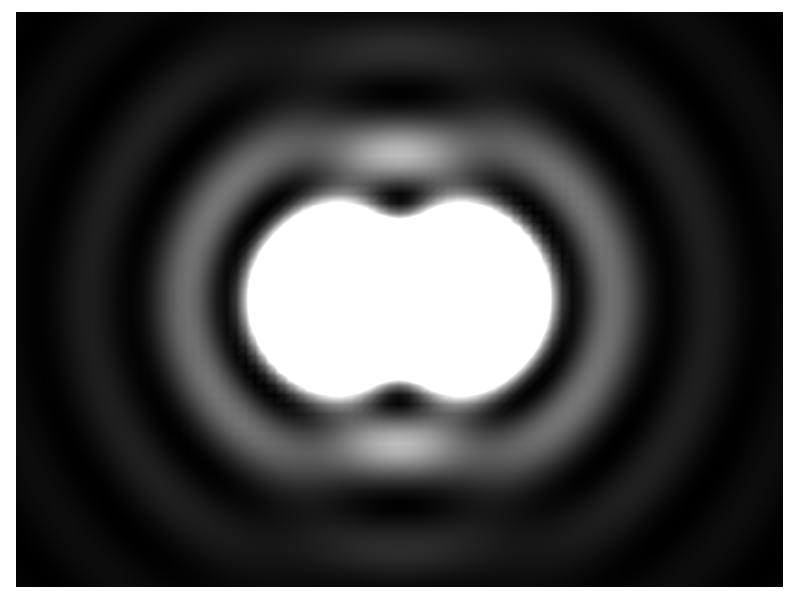
\includegraphics[width=4.7cm]{eiry-disk-1}\hfill
		\begin{tikzpicture}
			\begin{axis}[
				height	=	4.125cm,
				width	=	5.5cm,
				xlabel	=	{$x$, $\frac{\lambda}{D}$},
				ylabel	=	{$I/I_0$},
				ylabel shift	= -1 cm,
				]
				
				\addplot[smooth] table[x=x, y=e1]{data/eiry-disk-profile.txt};
			\end{axis}
		\end{tikzpicture}
		\caption{Диффракционное изображение от двух источников с разделением~$1.22\lambda/D$}
	\end{subfigure}\\
	\begin{subfigure}{\tw}
		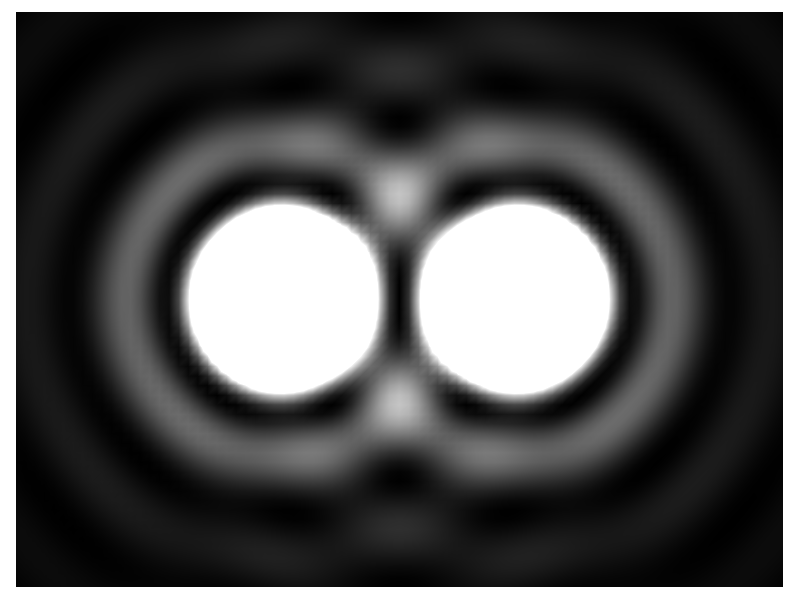
\includegraphics[width=4.7cm]{eiry-disk-2}\hfill
		\begin{tikzpicture}
			\begin{axis}[
				height	=	4.125cm,
				width	=	5.5cm,
				xlabel	=	{$x$, $\frac{\lambda}{D}$},
				ylabel	=	{$I/I_0$},
				ylabel shift	= -1 cm,
				]
				
				\addplot[smooth] table[x=x, y=e2]{data/eiry-disk-profile.txt};
			\end{axis}
		\end{tikzpicture}
		\caption{Диффракционное изображение от двух источников с разделением~$2 \cdot 1.22\lambda/D$}
	\end{subfigure}\\
	\begin{subfigure}{\tw}
		
\includegraphics[width=4.7cm]{eiry-disk-3}\hfill
		\begin{tikzpicture}
			\begin{axis}[
				height	=	4.125cm,
				width	=	5.5cm,
				xlabel	=	{$x$, $\frac{\lambda}{D}$},
				ylabel	=	{$I/I_0$},
				ylabel shift	= -1 cm,
				]
				
				\addplot[smooth] table[x=x, y=e3]{data/eiry-disk-profile.txt};
			\end{axis}
		\end{tikzpicture}
		\caption{Диффракционное изображение от двух источников с разделением~$3 \cdot 1.22\lambda/D$}
	\end{subfigure}
	\caption{}
\end{figure}

